\documentclass[tikz,border=10pt]{standalone}
% Scale s = 0.011713 cm/px, centre (394.5, 255.5) px, y flipped
\begin{document}
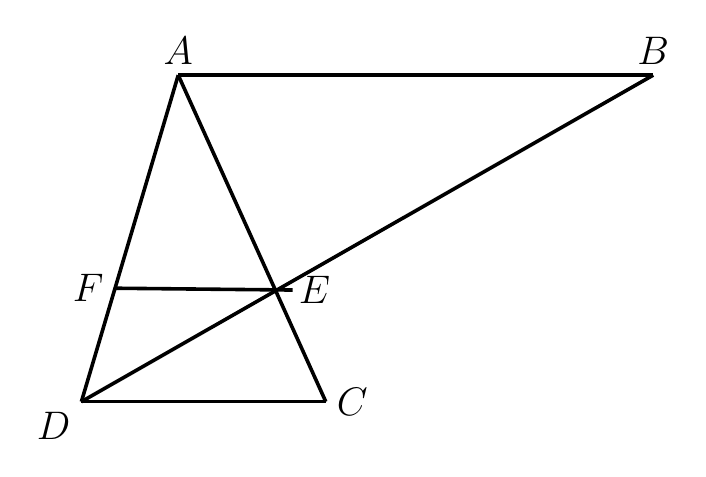
\begin{tikzpicture}[line width=1.3pt, line join=round]
  % Named coordinates (converted from pixels)
  \coordinate (A) at (-2.395,2.091);
  \coordinate (B) at (3.637,2.091);
  \coordinate (C) at (-0.521,-2.056);
  \coordinate (D) at (-3.625,-2.056);
  \coordinate (E) at (-1.154,-0.638);
  \coordinate (F) at (-3.203,-0.615);
  \coordinate (G) at (-0.943,-0.638); % FE extended to x=314 px

  % Solid segments
  \draw (A) -- (B);   % top AB
  \draw (D) -- (C);   % bottom DC
  \draw (A) -- (D);   % left leg AD (through F)
  \draw (B) -- (D);   % diagonal BD
  \draw (A) -- (C);   % diagonal AC
  \draw (F) -- (G);   % segment FE extended

  % Labels (outside the figure)
  \node[above] at (A) {\fontsize{13.5}{16.2}\selectfont $A$};
  \node[above] at (B) {\fontsize{13.5}{16.2}\selectfont $B$};
  % C: anchor west, level with vertex, just right of it
  \node[anchor=west] at (C) {\fontsize{13.5}{16.2}\selectfont $C$};
  \node[below left] at (D) {\fontsize{13.5}{16.2}\selectfont $D$};
  % E: anchor west, level with vertex; small xshift clears the FE stub end at x=314 px
  \node[anchor=west, xshift=0.15cm] at (E) {\fontsize{13.5}{16.2}\selectfont $E$};
  \node[left] at (F) {\fontsize{13.5}{16.2}\selectfont $F$};
\end{tikzpicture}
\end{document}